\documentclass[a4paper,12pt]{article}
\usepackage[ngerman]{babel}
\usepackage{ucs}
\usepackage{multirow}
\usepackage{xltxtra}
\usepackage[utf8x]{inputenc}
\usepackage{fontspec}
\usepackage[automark]{scrpage2}
\usepackage{eurosym}
\usepackage{graphicx}
\usepackage[paper=a4paper,left=25mm,right=25mm,top=25mm,bottom=25mm]{geometry}
\pagestyle{scrheadings}
\setmainfont[Mapping=tex-text]{Liberation Serif}
\clearscrheadfoot
\begin{document}
\ohead{Regelstand: \today}
\title{Regeln Fire Fighting Challenge 2018}

 \begin{center}

\includegraphics[width=0.5\textwidth]{logo.png}

\huge                      % Schriftgröße einstellen
\bfseries                   % Fettdruck einschalten
Regeln Fire Fighting Challenge 2018
  \end{center}
  Inhaltliche Änderungen im Vergleich zu den Regeln von 2017 sind \textbf{fett} markiert. Im Zweifel ist die Interpretation der Regeln durch die Schiedsrichter bindend.
\section{Aufgabe}
Baue und programmiere einen Roboter, der 4 zufällig verteilte Kerzen innerhalb eines durch eine schwarze
Linie abgegrenzten Feldes finden und löschen kann. Die erste Kerze ist von der Startposition aus sichtbar, die
anderen drei Kerzen sind durch Wände verdeckt. Die Gesamtpunktzahl ist umso höher, je schneller der
Roboter die Kerzen löschen kann.
\section{Wer kann teilnehmen?}
Teams aus \emph{2 bis 4 Spielern in unterschiedlichen Altergruppen}:
\begin{itemize}
	\item Altersgruppe 1 (Middle School): 10-13 Jahre
	\item Altersgruppe 2 (High School): 14-17 Jahre
	\item Altersgruppe 3 (Big Kids): 18-20 Jahre
\end{itemize}
\section{Materialanforderungen}
Autonomer Roboter basierend auf jeglicher Plattform, der maximal \euro{1500} kostet und den folgenden
Designanforderungen, die beim Check-In überprüft werden, entspricht:
\begin{itemize}
\item Der Roboter kann zeigen, dass sein System zum Löschen der Kerze durch eine Sensordetektion der Kerze
oder des sie umgebenden Kreises ausgelöst wird.
\item Wenn ein Ventilator zum Löschen eingesetzt wird, muss sicher gestellt sein, dass niemand durch diesen
verletzt werden kann.
\item Das Volumen des Roboter darf 65030 cm$^{3}$ nicht überschreiten.
\end{itemize}
Mehrere Sensoren und Prozessoren sind erlaubt.
\section{Spielfeld}
\begin{itemize}
\item Das Spielfeld ist ungefähr 2,4 × 3,6 m groß
\item Das Spielfeld wird durch weißes und schwarzes Klebeband abgegrenzt
\item Das weiße Klebeband an der Grenze ist 7,5 cm breit mit einem schwarzen, 2,5 cm
breiten Streifen in der Mitte
\item Die Kerzen und die Abdeckungen werden für jeden Durchgang zufällig auf dem
Spielfeld verteilt
\item Die Kerzen stehen in der Mitte eines weißen Kreises mit einem Durchmesser von
ungefähr 40,5 cm und einer schwarzen Linie mit 2,5 cm Breite, die ungefähr 2,5 cm
vom Rand entfernt ist.
\item Die Höhe der Kerze ist 25,5cm (gemessen vom Boden bis zum unteren Rand der
Flamme)
\item 3 Kerzen werden von jeweils einer Abdeckung verdeckt und eine Kerze ist vom Startpunkt des Roboters aus
sichtbar
\item Die Abdeckungen sind 46 cm breit und 43 cm hoch. Sie stehen auf Hohlstandfüßen, die 3,5 cm hoch sind und
über die komplette Breite des Holzes reichen.
\item Die Lichtbedingungen können sich im Laufe des Tages ändern. Der Roboter muss auf dieses natürliche
Problem vorbereitet sein
\end{itemize}
\begin{center}
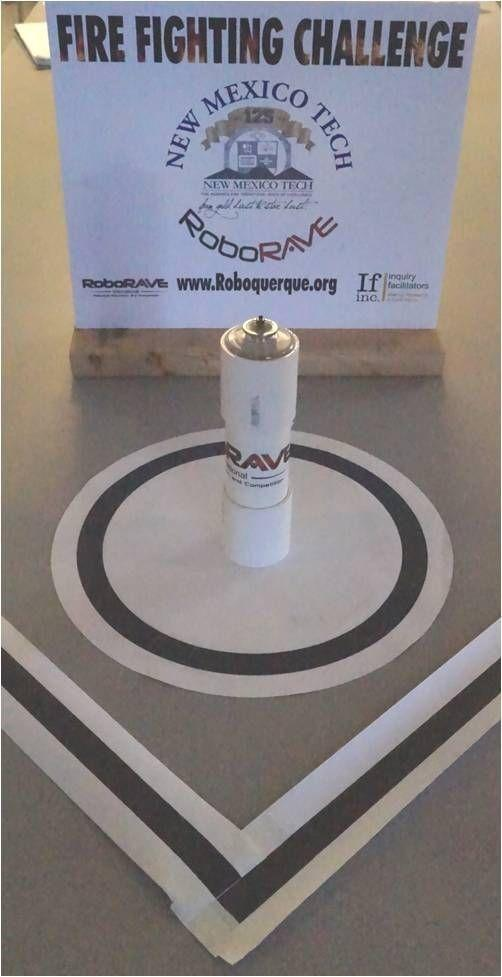
\includegraphics[width=0.4\textwidth]{candle.jpeg}
\end{center}
\section{Spielregeln}
\begin{itemize}
	\item Der Roboter startet an einem Punkt an der Grenzlinie, der vom Schiedsrichter bestimmt wird
	\item Zu Beginn ist eine Kerze von der Startposition des Roboters aus sichtbar
	\item Der Roboter hat 3 Minuten Zeit, um die 4 Kerzen zu löschen
	\item Nur Spieler dürfen den Roboter während eines Durchgangs berühren und bedienen
	\item Wenn ein Spieler den Roboter nach Beginn des Durchlaufs berührt, wird der Durchlauf abgebrochen und
	anhand der bereits gelöschten Kerzen bewertet
\end{itemize}
\section{Wertungszeitraum}
Die Art der Wertung der einzelnen Ergebnisse im Bezug auf den gesamten Wettbewerb wird am ersten Wettbewerbstag von den Schiedsrichtern bekanntgegeben. Änderungen der Wertungsmodalitäten bleiben den Schiedsrichtern vorbehalten.
\section{Punktevergabe}
Die Gesamtpunktzahl ist die Summe der Punkte, die während des Versuchs erzielt wurden und der
Sekunden, die verbleiben nachdem die letzte Kerze gelöscht wurde. Somit sind insgesamt bis zu 1000 reguläre Punkte plus 180 Punkte für Zeit möglich.

\section{Strafen}
\begin{itemize}
\item Das System zum Löschen der Kerze wird gestartet bevor ein Teil des Roboters den weißen Kreis überquert
hat. \textbf{(Kerze wird nicht gewertet)}
\item \textbf{Wenn eine Kerze gelöscht wurde obwohl der Roboter den weißen Kreis nicht überquert hatte erhöht sich die Punktzahl für die darauf folgende Kerze \emph{nicht}.}
\item Der Roboter berührt die Kerze während des Löschens. \emph{Der Löschvorgang gilt erst als beendet, wenn die
Flamme gelöscht ist und alle Teile des Roboters außerhalb des weißen Kreises sind}. (nur 50\% der Punkte für diese Kerze)
\item Kerzen die bereits gelöscht wurden zählen als Hindernisse und geben somit keine Strafpunkte wenn sie nach
dem Löschvorgang berührt werden.
\end{itemize}
\section{Punktetabelle}
\begin{center}
\begin{tabular}{|c|c|c|c|c|c|} \hline
	 & 1. Kerze & 2. Kerze & 3. Kerze & 4. Kerze  \\ \hline
	 Außerhalb Kreis & - & - & - & - \\ \hline
	Berührung & 50 & 100 & 150 & 200 \\ \hline
	Ohne Strafabzug & 100 & 200 & 300 & 400  \\ \hline
\end{tabular}
\end{center}
\end{document}